% !TEX root = main.tex
\chapter{Rocket Tests}

	MEOWTH II was tested at Peter Madsen's space laboratory in Copenhagen, on the 3rd to the 4th of May 2016 by Team Rocket of Navitas. The whole ordeal has spawned several articles, which the interested reader can find in appendix \ref{App:A}. A  complete logbook along with a firing procedure can be found in appendix \ref{App:B}.

	The test setup can be seen in figure \ref{fig:rocketpic}, and the first burn can be seen on the front page. The test stand consists of a metal fixture that holds the rocket in a vertical position, with the hydrogen--peroxide tank upright. The metal fixture keeps the rocket from moving under tests. Sandbags are placed on top in order to stop fast--moving shrapnel, in case of a complete engine destruction. Further safety instructions can also be found in appendix \ref{App:B}.

	The purpose of the experiments was to measure the variations in pressure throughout the rocket. The following will be an analysis of the data collected, along with a brief description of the sensors involved. A group consisting of three students also took video footage of the tests in order to analyze the rocket's shock diamonds, this will not be treated here, however.

	\section{Equipment}

	Eight pressure sensors were mounted on the rocket, ranging over three measurement frequencies: $\SI{250}{\Hz}$, $\SI{2000}{\Hz}$ and $\SI{10000}{\Hz}$. \fxnote{20khz??} One of each sensor was placed in both the rocket's mixing chamber and decomposition chamber. The two remaining sensors, a slow and a fast, were mounted by the hydrogen--peroxide tank. All sensors are connected to the data--logging software LabVIEW on a local computer, which was controlled by an external computer placed inside the safety--submarine.

	Two manometers were placed before and after the pressurization valve, in order to manually check the tank's pressure before ignition.


% Testing of the rocket engine ensued at "Raketmadsens Rumlaboratorium" in Copenhagen on the 3rd to the 4th of may 2016. The tests were carried out by me in company by my advisor Gorm Bruun Andresen, and seven other students from Navitas.
%

%
% 	The control computer should be replaced by a microcontroller, such as an arduino or raspberry pi. As of this project, the data bandwidth is too low in either alternative, but it is a viable solution in the near future.
%
% 	In order to reduce reload time, adding more piping to the christmas tree is necessary, as air leaving the \chem{H_2 O_2} tank flows back, spilling the \chem{H_2 O_2} concentration out of the funnel. When a suitable final design is done, welding the pieces together is a superior alternative to using bolts and nuts. Welding removes any chance hydrogenperoxide leaking, damaging the rocket and measurement equipment.
%
% 	The rocket's arming and controlpad needs to be set up in a smarter, more convenient way. The ideal setup is to have a single controlbox, that when starts data-collection as soon as the rocket is armed, and notes when it is fired. This would allow everything to be controlled from a single box, with measurements being saved to a raspberry pi situated at the base of the rocket. Data can then instantaneously be read from a secondary computer through cable or wireless connection. As the rocket's final destination is space, continuously improving data-transfer and making the rocket an individual unit is paramount.
%
% Removing additional noise from measurements can easily be done avoiding ground-loops. The ignition controlpad was grounded differently than the other equipment, which introduced another way for electricity to run to ground.
%
% \section{Results}
%
% A total of ten measurements were collected at every test. The most essential is the Piezoelectric pressure sensors located at the front. The simulation calculates the pressure after the combustion chamber, and at the nozzle's exit.
%
% \begin{figure}
% 	\centering
% 	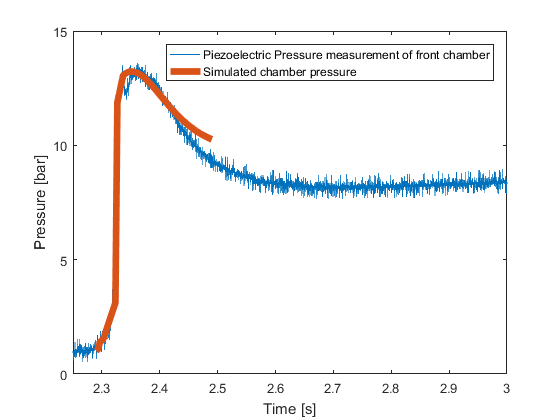
\includegraphics[width=\textwidth]{peakBurn2wsim}
% 	\caption{The second burn's front chamber peak, as found by the Piezoelectric pressure sensor. Plotted on top is the simulation created in this bachelor's thesis.}
% 	\label{fig:peakBurn2wsim}
% \end{figure}
%
% The experimental and simulation results are seen in figure \ref{fig:peakBurn2wsim}, where the blue line is the experimental results, and the red is the simulated pressure. The simulation assumes no combustion until a temperature of $\SI{220}{\celsius}$, at which all of the oxygen inside the combustion chamber is instantly consumed, followed by a steady burning phase. The instantaneous combustion looks like an explosion, as more oxygen is available at this point than at any other. The experimental front pressure dips shortly after initial combustion, which may be due to a shockwave moving through the rocket, forcing new oxygen from flowing to the grain's surface for a short period of time. The pressure then drops rapidly to a steady state, where the simulation ends just prior. The abrupt ending is due to a bug in the current version of the simulation software EES, which crashes after a certain number of iterations. Future versions may allow the calculation of the steady state. Take note of the simulation's timescale, as the duration of the peak is very small, almost only two tenths of a second.
%
%
% \begin{figure}
% 	\centering
% 	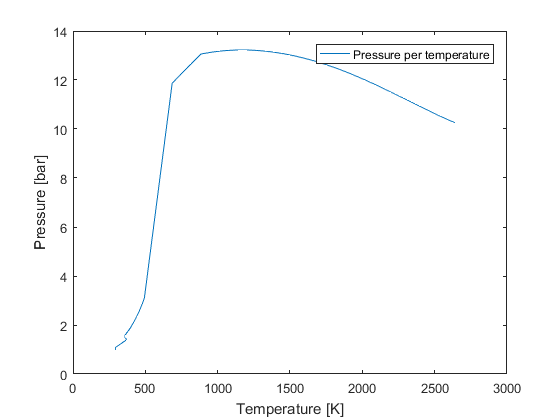
\includegraphics[width=\textwidth]{PperTsimonly}
% 	\caption{Pressure per temperature plotted over the simulated timespan in figure \ref{fig:peakBurn2wsim}. As the temperature rises, the pressure falls.}
% 	\label{fig:pressurepertemp}
% \end{figure}
